\section{Abstraction}
\label{section:abstraction}

When a segment is produced in the segmentation process, it is abstracted to a single symbol in the superordinate abstraction layer.  Since each dimension is composed of both an alphabet of symbols and a conceptual space in which those symbols live, a memory sequence is at once a segment of symbols in the sequential memory as well as a trajectory through the corresponding conceptual space in the semantic memory \citep{wiggins2019learning}. Since here we will utilize the formalism of finite-dimensional Hilbert spaces to model conceptual spaces, this trajectory corresponds to a time-parametric curve in a high-dimensional space.

\subsection{Fourier Transform}
\label{section:fourier-transform}

In the abstraction process, we would like to produce a spectral representation of a segment.  Here, we will apply the discrete Fourier transform (DFT) operator \citep{cooley1965algorithm} to the discrete trajectory (see equation \ref{equation:discrete-fourier-transform}), taking it from the time-domain $n$ to the frequency-domain $k$.  Though there are other spectral operators, there is evidence, especially in the auditory domain, that the brain operates on frequency transformations of time-varying signals from the Organ of Corti \citep{moore2012introduction}, and so it is employed here.  

\begin{equation}
  \label{equation:discrete-fourier-transform}
  \mathcal{F}_D [x_n] = X_k = \sum_{n=0}^{N-1} x_n e^{-\frac{i 2 \pi}{N} kn}
\end{equation}

By taking the Fourier transform (equation \ref{equation:fourier-transform}) of a time-varying signal $f(t)$, we produce the frequency-domain signal $F(\xi)$ for each orthogonal frequency.  So by taking the Fourier transform of a curve in a Hilbert space, we end up with a spectral representation of that curve.  The abstraction process will then consist of taking the Fourier transform of a trajectory through a Hilbert space, and then viewing the resulting frequency-domain signal as a point in the superordinate space.

\begin{equation}
  \label{equation:fourier-transform}
  \mathcal{F} [f(t)] = F(\xi) = \int_{-\infty}^\infty f(t) e^{-i 2 \pi \xi t} dt
\end{equation}

\subsection{Tensor Rank Promotion}
\label{section:tensor-rank-promotion}

The Fourier transform is an integral operator on Hilbert spaces \citep{kennedy2013hilbert}.  Since operators, by definition, take a function as input and produce a function as output, when thinking in terms of finite-dimensional Hilbert spaces, an operator will take the input from one domain to another, but will not change the shape of that input.  For example, if each point is represented as a vector, a sequence of those points would be a vector of vectors, i.e. a matrix.  Since we view the result of the Fourier transform as a point in the superordinate space, in our example, the point is now represented as a matrix.  Therefore, the result of abstracting a trajectory of points in a subordinate layer is a point in the superordinate space with one higher rank.  Hence, each level of abstraction promotes the rank of its constituent tensors by one. 

To clarify the first few stages of this process, consider Figure \ref{figure:tensor-rank-promotion}. The \textit{Element} row represents the constituent elements of layer $\alpha$.  The \textit{Trajectory} row strings those elements together, and the \textit{Spectral} row shows the shape of the spectral representation of that trajectory after the Fourier transform.  This spectral representation then becomes the constituent element of the superordinate abstraction layer $\alpha+1$.

We begin at the base abstraction layer with a space filled with the raw discrete scalar signal values for each moment of time.  By lining up these values and taking their Fourier transform, the resulting spectral representation is a vector.  This spectral representation is placed into the $\alpha=1$ abstraction layer, whose space is filled with points representing the frequencies of a signal of a short moment of time.  These points are vectors (rank 1 tensors) that, when strung together into a trajectory, form a matrix.  By taking the Fourier transform of this matrix and viewing the result as a point in the superordinate abstraction layer, that upper layer is now composed of points represented as matrices (rank 2 tensors).  Again, we string these points together as a trajectory, but now forming a cube.  By taking the Fourier transform, and viewing it as a point in the superordinate layer, that layer is now composed of points represented as cubes (rank 3 tensors). Repeating this process, we then get hypercubes of increasing rank at each layer of abstraction.  In this manner, the rank of a representative tensor increases by one for each layer of abstraction.

Unfortunately, this leads to an exponential explosion in the number of elements constituting a point in a given layer.  Formally, the number of elements is $r^\alpha$, where $r$ is the resolution of interpolation (see section \ref{section:interpolation}), and $\alpha$ is the level of abstraction.  Though this is not a problem in theory, it has consequences in terms of implementation.

\begin{figure}
  \centering
  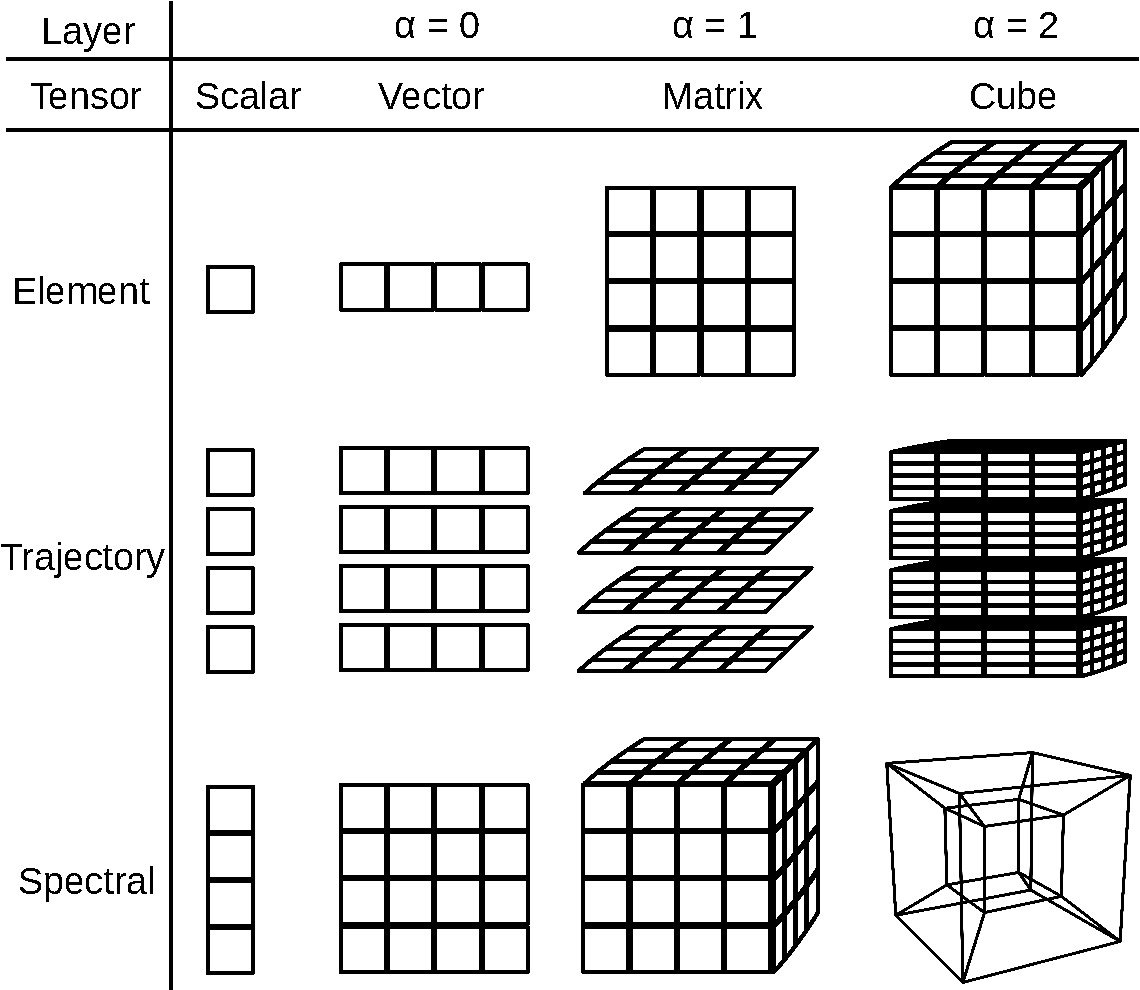
\includegraphics[width=\linewidth]{fig/tensor-rank-promotion.pdf}
  \caption{An illustration of tensor rank promotion for the first 4 levels of abstraction, using an interpolation resolution $r = 4$.  }
  \label{figure:tensor-rank-promotion}
\end{figure}

\subsection{Element-wise Independence}
\label{section:elementwise-independence}

When performing the Fourier transform on a tensor of any rank, it should be noted that each component in the tensor is independent from every other component.  Though this is not necessarily true of tensors in general, due to the particular hierarchical construction of these spaces by means of the DFT, each component is decoupled from the rest.  Starting at the bottom, the time-domain sound signal is transformed into a frequency-domain signal of coefficients in independent frequency bins.  It is this independence that allows us to represent the short-term frequency signal as a point with those frequency bins as dimensions.  Performing the DFT on the trajectory of frequency vectors results in independent frequency bins filled with vectors that possess independent entries, meaning all elements are independent one another.

Hierarchically performing the DFT at each abstraction layer on tensors with independent elements results in higher rank tensors with independent elements.  This element-wise independence of the tensor means that the DFT should be taken element-wise -- that is, across the base "time" axis -- since all other cross-component terms would involve orthogonal dimensions.

\subsection{Frobenius Norm}
\label{section:frobenius-norm}

The norm chosen for this implementation is the Frobenius norm \citep{horn1990norms}.  This norm corresponds with the familiar Euclidian norm, but since we are operating more generally on tensors, and not just vectors, the Frobenius norm is employed instead.  This norm corresponds to a flat space where each dimension behaves linearly and equally in relation to the other dimensions.  The Frobenius norm is intuitive for visualizing the space, and so serves as a good norm to begin exploration.  Future research will investigate different inner products and their induced norms to impose different geometries on the representations.

\begin{equation}
  \label{equation:frobenius-norm}
  \|A\|_F = \sqrt{\sum_{i=1}^m \sum_{j=1}^n |a_{ij}|^2}
\end{equation}

In equation \ref{equation:frobenius-norm}, the Frobenius norm is shown for a matrix.  One can then imagine that for a cube, there would be three summations, four summations for a hypercube, and so on.  Therefore, the Frobenius norm comes to be a sum over each element of the tensor.
